%  article.tex (Version 3.3, released 19 January 2008)
%  Article to demonstrate format for SPIE Proceedings

%  The following commands have been added in the SPIE class 
%  file (spie.cls) and will not be understood in other classes:
%  \supit{}, \authorinfo{}, \skiplinehalf, \keywords{}
%  The bibliography style file is called spiebib.bst, 
%  which replaces the standard style unstr.bst.  

%----------------------------------------------------------------------------------------------------
% PACKAGES
%----------------------------------------------------------------------------------------------------

\documentclass[]{spie}  % use for US letter paper
\usepackage{comment}
%%\documentclass[a4paper]{spie}  %>>> use this instead for A4 paper
%%\documentclass[nocompress]{spie}  %>>> to avoid compression of citations
\usepackage[]{graphicx}
\usepackage{epsfig}		% TeX will automatically convert eps --> pdf in pdflatex	
\usepackage{epstopdf}
\usepackage{caption}
\usepackage{subcaption}
\usepackage{multirow}
\usepackage{array}
\usepackage{tabularx}
\usepackage{enumerate}
\usepackage{amsmath}
\usepackage{amsfonts}
\usepackage{bbm}
\usepackage[mathcal]{euscript}
\usepackage{mathtools}

\setcounter{MaxMatrixCols}{14}
\DeclarePairedDelimiter\floor{\lfloor}{\rfloor}
%\renewcommand{\baselinestretch}{1.65}   %>>> 1.65 for double spacing, 1.25 for 1.5 spacing 
%\addtolength{\voffset}{9mm}   %>>> moves text field down

%----------------------------------------------------------------------------------------------------
% TITLE
%----------------------------------------------------------------------------------------------------

\title{An Online Visual Loop Closure Detection Method for Indoor Robotic Navigation} 

%----------------------------------------------------------------------------------------------------
% AUTHORS
%----------------------------------------------------------------------------------------------------

\author{
Can Erhan\supit{a}, 
Evangelos Sariyanidi\supit{b}, 
Onur Sencan\supit{c}, 
Hakan Temeltas\supit{c}
\skiplinehalf
\supit{a}Istanbul Technical University Mechatronics Engineering Department, Maslak 34469, Istanbul, Turkey; 
\supit{b}Centre of Intelligent Sensing, Mile End Road, E1 4NS, London, U.K.;
\supit{c}Istanbul Technical University Control and Automation Engineering Department, Maslak 34469, Istanbul, Turkey
}

\authorinfo{Further author information: \\
Can Erhan: E-mail: erhanc@itu.edu.tr \\  
Evangelos Sariyanidi: E-mail: e.sariyanidi@eecs.qmul.ac.uk \\
Onur Sencan: E-mail: osencan@itu.edu.tr \\  
Hakan Temeltas: E-mail: hakan.temeltas@itu.edu.tr}
% when using amstex, you need to use @@ instead of @
 
% uncomment following for page numbers
% \pagestyle{plain}    
% uncomment following to start page numbering at 301 
% \setcounter{page}{301} 
 
 %----------------------------------------------------------------------------------------------------
% ABSTRACT
%----------------------------------------------------------------------------------------------------
 
 \begin{document} 
\maketitle 

\begin{abstract}
Visual loop closure detection problem is an active research area for indoor environments, where the global position information is missing and the localization information is highly dependent on odometry sensors. In this paper, we propose an enhanced loop closure method based on unsupervised visual landmark extraction by means of quantized local Zernike moments. In contradistinction to the previous methods, our approach uses additional depth information to extract Zernike moments. Zernike transform is an effective tool for referring to the certain distinctive areas on the image patches. Therefore, it is a suitable method to represent locations in a sparse manner.  In order to find out the similarity between two locations, we propose a straightforward function that contains the detection confidences of the image and the landmark coordinates in 3D. Recognition of the previously visited and unvisited locations are also considered in the framework. Examplary results and the practical implementation case of the method are also given with the data gathered on the testbed using a depth camera (Kinect) mounted differential drive autonomous ground vehicle. The results are referred as a successful, high-fidelity online method for visual place recognition as well as to close navigation loops, which is a crucial information for the well known simultaneously localization and mapping(SLAM) problem. The algorithm is tested in three different datasets of different lighting conditions. Additional depth information beside the actual image increases the detection rate especially in dark. 
\end{abstract}

\keywords{Loop closure, depth map, zernike moments,  computer vision}

%----------------------------------------------------------------------------------------------------
% INTRODUCTION
%----------------------------------------------------------------------------------------------------

\section{INTRODUCTION}

In mobile robotics, autonomous navigation is an active research area especially for the indoor environments, where the global position information is missing and the localization information is highly dependent on odometry sensors. One of the major problems connected to robotic navigation is Simultaneous localization and mapping (SLAM) which still remains as an assertive problem in a lot of ways. Loop closing is defined as the correct identification of previously visited location in terms of SLAM. Information that is gathered from various data sources including LIDARs, RADARs, stereo and monocular cameras\cite{williams08iros, 5650234} is highly utilized in loop closure detection. With the recent development of visual sensor technologies, the loop closure detection became a problem that is open for research in the field of computer vision.

Visual loop closing techniques can be categorized into three main parts\cite{Williams09}: Image-to-image and image-to-map, map-to-map techniques. Loop closure estimations\cite{sariyanidi_spie13}  are cast by matching images. Most of image-to-image techniques that rely on salient image patches, use small, low-level features such as SURF\cite{springerlink:10.1007/11744023_32} extracted from the whole image \cite{sariyanidi_iv, HoNewmanCIRA2005, CumminsNewmanIJRR08}. One of the widely used methods in visual place recognition problem is the Bag of Words\cite{1238663} method. Also, there are some studies that uses additional depth information\cite{kerl2013-IROS} in loop closure problems.More information related to visual loop closing approaches can be found on the relevant survey \cite{Williams09}.

In this paper, we present an enhanced loop closure method based on image-to-image matching with the additional depth information in indoor environments. Specifically, we adopt visual place recognition without using any metrical information such as rotation and exact location to correctly identify the previously visited location. This technique is quite simple because of its low computational complexity, and performs in real-time with high loop closing accuracy. 

The technique we implement relies on discrete Complex Zernike Moments (CZMs) in 2-dimensional space. They are extracted using a set of complex polynomials which form a complete orthogonal radial basis functions defined on the unit disc. These moments are used to represent shape information inside the image within the context of image processing. To make the image description more robust, the ZMs of the input image is calculated in local manner. In this study, the ZMs are extracted from both the greyscale and depth images separately and concatenated sequentially to create ultimate feature vector.

The locations are represented with the histograms of their images. Detecting loop closing events can be considered as a machine learning problem which number of classes expands continuously when a new unseen location comes. We utilized Nearest Neighbour (NN) algorithm to classify locations by which the distance metric is the regular $L_1$ a.k.a. Manhattan distance that is one of the simplest distance metric available. In other words, the image which distance between the input image is minimum closes the loop, if the distance is lower than the predefined threshold value. 

In the following sections, a brief introduction about the methodology is explained first, and then the experiments and datasets are shown, and finally results are presented. 

%----------------------------------------------------------------------------------------------------
% METHODOLOGY
%----------------------------------------------------------------------------------------------------

\section{METHODOLOGY}
\label{sec:method}

As it was mentioned earlier, the presented loop closing approach relies on calculating the Zernike Moments of partitioned image blocks across the input image in a local manner. 

The whole image representation is constructed as follows. Firstly, the ZMs of each subimage that were obtained by partitioning the input image is calculated. After that, the calculated complex moments are coarsely quantized by keeping only the sign of the real and imaginary components and ignoring the rest of the information. Next, the quantized binary data is combined linearly by weighting each of them to convert them into integers. Finally, the integers values are coded as histograms.

%%% PARTITIONED IMAGE
\begin{figure}[!htb]
        \centering
         % trim parameters by order: left, bottom, right, top
        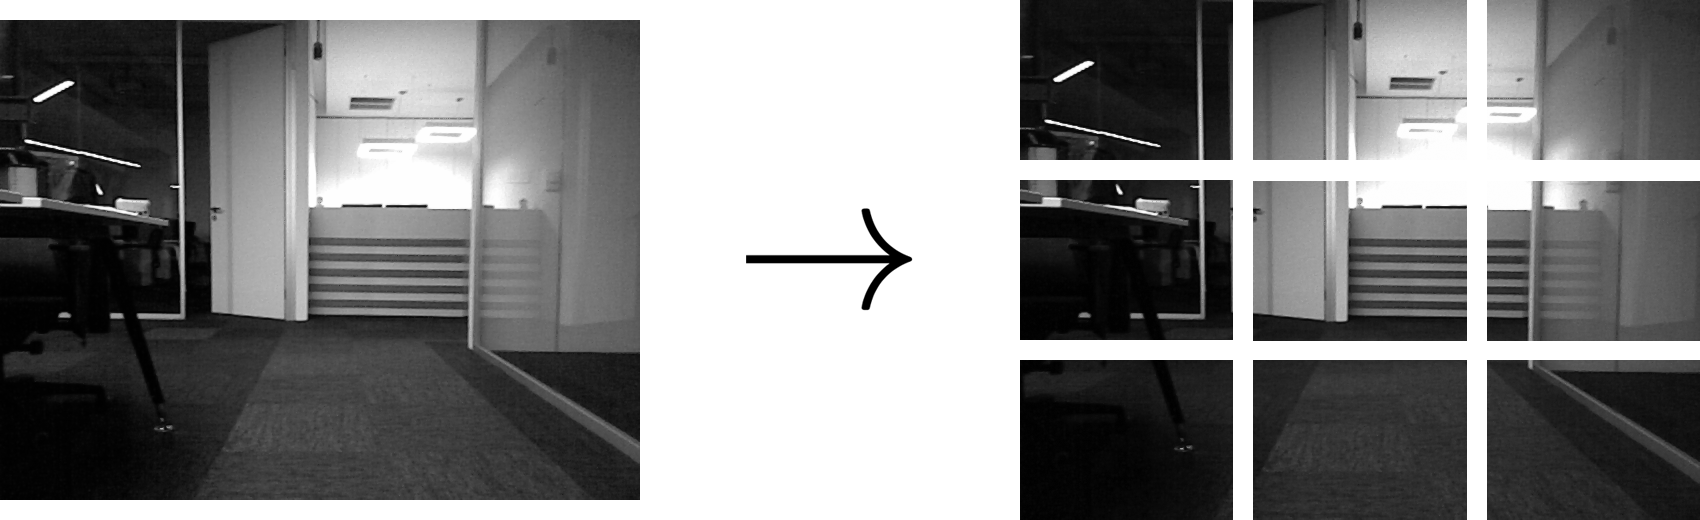
\includegraphics[trim = 0mm 0mm 0mm 0mm, clip, height=3cm]{figures/divided_image.png}    
        \vspace{3mm}
        \caption{Image partitioned into blocks by k = 3}
        \label{fig:divided_image}
\end{figure}

\subsection{Extraction of Quantized Local Zernike Moments} 

The Complex Zernike Moments (ZM) of an image are used to represent the image on the 2-dimensional complex subspace. They are extracted using a set of complex polynomials which form a complete orthogonal radial basis functions defined on the unit disc. The coefficients in this complex subspace describe the holistic shape information within the image. 

The Complex Zernike Moments of an image $f(i,j)$ are calculated as follows:

\begin{equation}
\label{eq:global_zernike}
Z_{nm} = \frac{n+1}{\pi}\sum^{N-1}_{i=0}\sum^{N-1}_{j=0}f(i,j)V^\star(\rho_{ij},\theta_{ij})\Delta
x_i\Delta y_j, \\
\end{equation}
where $x_i$, $y_j$ stand for the image coordinates, $\quad\rho_{ij}=\sqrt{x_i^2+y_i^2}$ and $\quad\theta_{ij} = \tan^{-1}\frac{y_j}{x_i}$ are the polar coordinates of the image, $n$ defines the order of the ZM and $m$ stands for the number of repetitions. The constraint between $n$ and $m$ is stated that $|m|\leq n$, and $n-|m|$ must be even. Therefore, the number of components with respect to moment order $n$ is calculated as follows:

\begin{equation}
K(n) =
\begin{cases}
  \frac{n(n+2)}{4} &\text{if $n$ is even} \\ 
  \frac{(n+1)^2}{4} &\text{if $n$ is odd}.
\end{cases}
\label{eq:num_moms}
\end{equation}

In order to extract ZMs in local manner, the input image is divided by $k\times k$-sized subimages in which $k$ is a predefined partitioning parameter. If the image is not divided by $k$ perfectly, the rest of the part is simply ignored. The set of images obtained from partitioning are flatten into a  $k^2\times 1$-sized single column in row-major order for more straightforward representation.

Consider that the input image $\mathbf{I}_{p\times q}$ is a combination of subimages $I_{ij}$:

\begin{equation}
\mathbf{I}_{p\times q} = \begin{bmatrix}
 I_{11} & \hdots & I_{1Q} \\
 \vdots & \ddots & \vdots \\
 I_{P1} & \hdots & I_{PQ} 
 \end{bmatrix}
 \longrightarrow
 \begin{bmatrix}
 I_{11} \\
 \vdots \\
 I_{1Q} \\
 \vdots \\
 I_{P1} \\
 \vdots \\
 I_{PQ}
 \end{bmatrix}
 \label{eq:divided_mat}
\end{equation}
where $P=\floor*{^p/_k}$ and $Q=\floor*{^q/_k}$. An exemplar input image partitioned into subimages is shown in Figure \ref{fig:divided_image}. The $Z_{nm}$ of the input image can be considered as the transformation of the subimages in (\ref{eq:divided_mat}) individually. This transform is applied to subimages with all $n$ and $m$ values according to its order. Lastly, the ZMs computed from transformed subimages are collected into a new matrix as follows:

\begin{equation}
\mathbf{Z} ( \mathbf{I}_{p\times q} )= 
\begin{bmatrix}
\mathbf{Z}(I_{11}) \\
  \vdots \\
\mathbf{Z}(I_{1Q}) \\
  \vdots \\
\mathbf{Z}(I_{P1}) \\
  \vdots \\
\mathbf{Z}(I_{PQ}) \\
 \end{bmatrix}
 \longrightarrow
 \begin{bmatrix}
Z_{00}(I_{11}) & \hdots & Z_{nm}(I_{11}) \\
  \vdots  & & \vdots \\
Z_{00}(I_{1Q}) & \hdots & Z_{nm}(I_{1Q}) \\
  \vdots  & & \vdots \\
Z_{00}(I_{P1}) & \hdots & Z_{nm}(I_{P1}) \\
  \vdots  & & \vdots \\
Z_{00}(I_{PQ}) & \hdots & Z_{nm}(I_{PQ}) \\
 \end{bmatrix} = 
 \begin{bmatrix}
a_{00}^{11} + \mathbf{i}b_{00}^{11} & \hdots & a_{nm}^{11} + \mathbf{i}b_{nm}^{11} \\
  \vdots  & & \vdots \\
a_{00}^{1Q} + \mathbf{i}b_{00}^{1Q} & \hdots & a_{nm}^{1Q} + \mathbf{i}b_{nm}^{1Q} \\
  \vdots  & & \vdots \\
a_{00}^{P1} + \mathbf{i}b_{00}^{P1} & \hdots & a_{nm}^{P1} + \mathbf{i}b_{nm}^{P1} \\
  \vdots  & & \vdots \\
a_{00}^{PQ} + \mathbf{i}b_{00}^{PQ} & \hdots & a_{nm}^{PQ} + \mathbf{i}b_{nm}^{PQ} \\
 \end{bmatrix}.
 \label{eq:lzm_op}
\end{equation}

Therefore, $k^2\times K(n)$-sized complex coefficient matrix is obtained. In order to facilitate the representation of the data and to reduce the size of the descriptor vector, a coarse quantization takes place at this step. First, the complex numbers are decoupled as real and imaginary components, then the sign of each matrix element is taken to binarize the decoupled $k^2\times 2K(n)$-sized matrix as follows:

\begin{equation}
\mathbf{Z} ( \mathbf{I}_{p\times q} )
 \longrightarrow
 \begin{bmatrix}
a_{00}^{11} & b_{00}^{11} & \hdots & a_{nm}^{11}  & b_{nm}^{11} \\
  \vdots  & \vdots & & \vdots  & \vdots\\
a_{00}^{1Q} & b_{00}^{1Q} & \hdots & a_{nm}^{1Q}  & b_{nm}^{1Q} \\
  \vdots  & \vdots & & \vdots  & \vdots\\
a_{00}^{P1} & b_{00}^{P1} & \hdots & a_{nm}^{P1}  & b_{nm}^{P1} \\
  \vdots  & \vdots & & \vdots  & \vdots\\
a_{00}^{PQ} & b_{00}^{PQ} & \hdots & a_{nm}^{PQ}  & b_{nm}^{PQ} \\
 \end{bmatrix}
  \longrightarrow
  \begin{bmatrix}
sgn(a_{00}^{11}) & sgn(b_{00}^{11}) & \hdots & sgn(a_{nm}^{11}) & sgn(b_{nm}^{11}) \\
  \vdots  & \vdots & & \vdots  & \vdots\\
sgn(a_{00}^{1Q}) & sgn(b_{00}^{1Q}) & \hdots & sgn(a_{nm}^{1Q}) & sgn(b_{nm}^{1Q}) \\
  \vdots  & \vdots & & \vdots  & \vdots\\
sgn(a_{00}^{P1}) & sgn(b_{00}^{P1}) & \hdots & sgn(a_{nm}^{P1}) & sgn(b_{nm}^{P1}) \\
  \vdots  & \vdots & & \vdots  & \vdots\\
sgn(a_{00}^{PQ}) & sgn(b_{00}^{PQ}) & \hdots & sgn(a_{nm}^{PQ}) & sgn(b_{nm}^{PQ}) \\
 \end{bmatrix}
 \label{eq:lzm_binary}
\end{equation}
where $sgn(\bullet)$ is the signum function. According to (\ref{eq:global_zernike}), $Z_{nm}$ with $m = 0$ is omitted since their imaginary components turn out to be constantly equal to zero. 

The next step is representing the binary matrix shown in (\ref{eq:lzm_binary}) with histograms. Using the binary values for the overall image representation is not a practical solution. Describing binary data with histograms are more common solution to obtain the image representation. As the methodology described so far, $k^2\times 2K(n)$-sized binary matrix is extracted. Each row of this matrix is linearly combined by weighting each of them as a power of $2$. Hence a column vector $\mathbf{C}$ is obtained with integer values ranging between $0$ and $2^{2K(n)-1}-1$:

\begin{equation}
\mathbf{C} = 
\begin{bmatrix}
c_{j}
\end{bmatrix}=
  \begin{bmatrix}
sgn(a_{00}^{11}) & sgn(b_{00}^{11}) & \hdots & sgn(a_{nm}^{11}) & sgn(b_{nm}^{11}) \\
  \vdots  & \vdots & & \vdots  & \vdots\\
sgn(a_{00}^{1Q}) & sgn(b_{00}^{1Q}) & \hdots & sgn(a_{nm}^{1Q}) & sgn(b_{nm}^{1Q}) \\
  \vdots  & \vdots & & \vdots  & \vdots\\
sgn(a_{00}^{P1}) & sgn(b_{00}^{P1}) & \hdots & sgn(a_{nm}^{P1}) & sgn(b_{nm}^{P1}) \\
  \vdots  & \vdots & & \vdots  & \vdots\\
sgn(a_{00}^{PQ}) &sgn(b_{00}^{PQ}) & \hdots & sgn(a_{nm}^{PQ}) & sgn(b_{nm}^{PQ}) \\
 \end{bmatrix}
 \begin{bmatrix}
2^0 \\
2^1 \\
 \vdots \\
 \vdots \\
 \vdots \\
 2^{2 K(n)-2} \\
 2^{2 K(n)-1}
 \end{bmatrix}
 \label{eq:lzm_coded}
\end{equation}

Finally, the histogram is defined that consists of $2^{2K(n)-1}$ bins, and each bin is filled with the number of occurrences of the integers in $\mathbf{C}$. Therefore, the input image $I_{p\times q}$ is described with a histogram of length of $2^{2K(n)-1}$.

%----------------------------------------------------------------------------------------------------
% EXPERIMENTS
%----------------------------------------------------------------------------------------------------

\section{EXPERIMENTS}

The method implemented in this paper has been evaluated on three datasets which lighting conditions are different from each other. The tests are done with either using gray and depth images separately or using both of them. After that, the difference matrices are calculated to examine the results. Nearest Neighbour (NN) algorithm is utilized to classify the new locations and the distance metric is $L_{1}$.

The method described in Section \ref{sec:method} has basically two parameters that must be adjusted. One of them is $k\times k$ the size of subimages that the input image partitioned by in (\ref{eq:divided_mat}) and the other one is $n$ the order of the Zernike polynomials. During the experiments, the parameter set is selected as $k=30$ and $n=2$. Then the quantized $k\times k$-sized matrix obtained from the input image is divided into $5\times 5$ equal-sized non-overlapping subregions. The histograms of each subregion are simply concatenated to compose the feature vector of an image. In order to construct the ultimate feature vector containing both gray and depth images, each feature vectors obtained from both images are also concatenated.

\subsection{Benchmark Datasets}

In order to measure loop closing performance of the algorithm in different illumination levels, three different datasets are created in an indoor environment by using Kinect sensor which can grab both RGB and depth images at the same time. The lighting conditions in the datasets are bright, dim and dark in which both depth and RGB images are captured. The exemplary images belonging to different datasets are shown in Figure \ref{fig:dataset}. In some cases, the line of sight of the Kinect is not enough to capture the depth information for distances above $10m$. Thus, some of the depth images are unreliable.

The images in the datasets are acquired via Kinect mounted moving platform and pointed in the direction of the displacement with approximate speed 0.25m/s. Also, the rectangle-shaped trajectory of the three datasets is almost the same as the others to compare their performances correctly. There are two loops that contain around 1000 frames per loop in each dataset, first one is used for discovering and the second for evaluating. To create the ground truth, the locations which corresponds to approximately 10 sequential frames are annotated manually. 

% BENCHMARK DATASETS
\begin{figure}[!htb]
        \centering
        
        %%% BRIGHT 
        \begin{subfigure}[b]{0.27\textwidth}
        \centering
         % trim parameters by order: left, bottom, right, top
        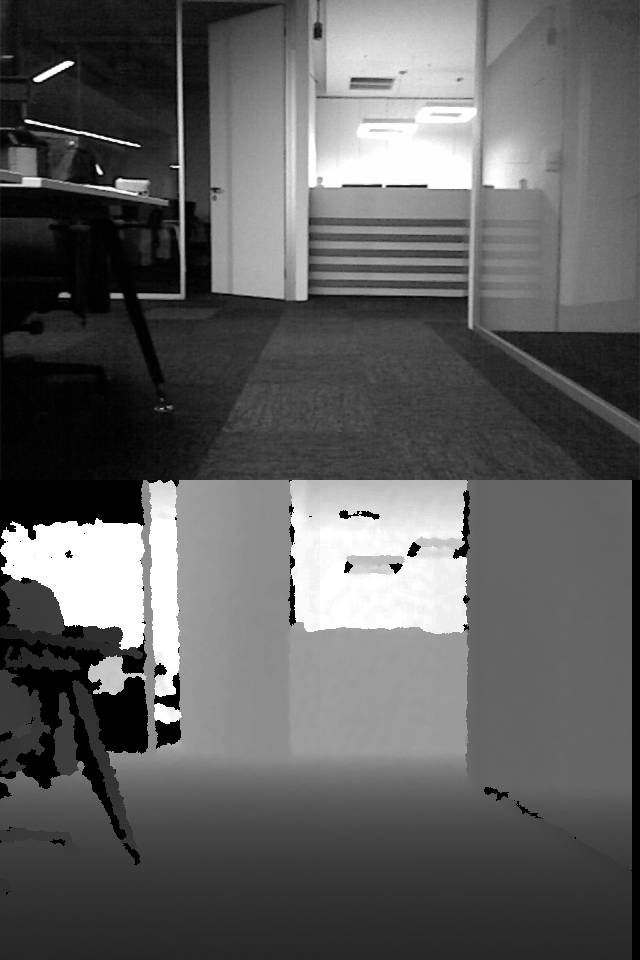
\includegraphics[trim = 0mm 0mm 0mm 0mm, clip, width=\textwidth]{figures/dataset_bright.png}    
        \caption{Bright}
        \label{subfig:dataset_bright}
        \end{subfigure}
        ~ 
        %%% DIM 
        \begin{subfigure}[b]{0.27\textwidth}
        \centering
         % trim parameters by order: left, bottom, right, top
        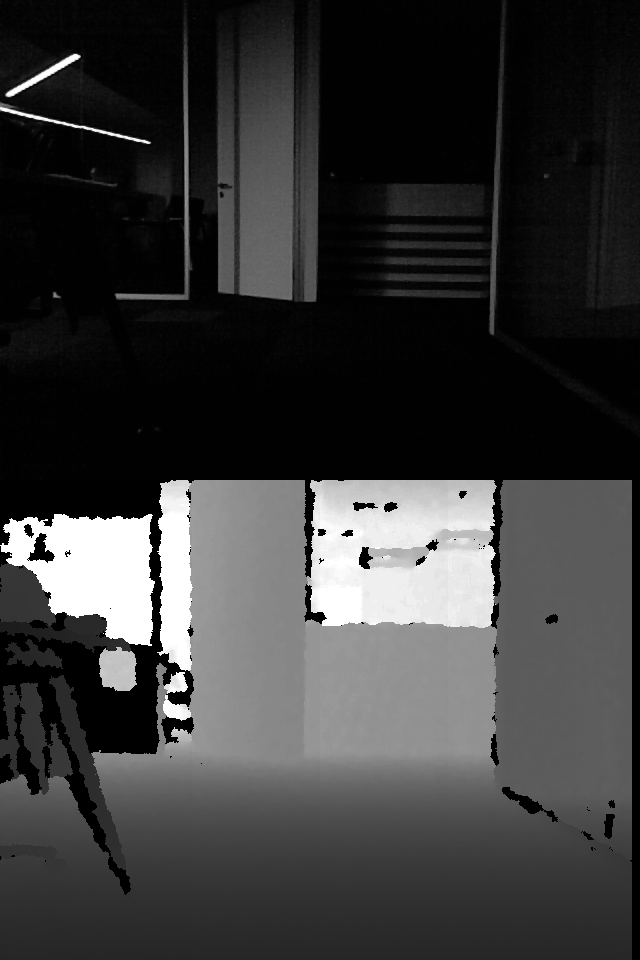
\includegraphics[trim = 0mm 0mm 0mm 0mm, clip, width=\textwidth]{figures/dataset_dim.png}    
        \caption{Dim}
        \label{subfig:dataset_dim}
        \end{subfigure}
         ~ 
        %%% DARK
        \begin{subfigure}[b]{0.27\textwidth}
        \centering
         % trim parameters by order: left, bottom, right, top
        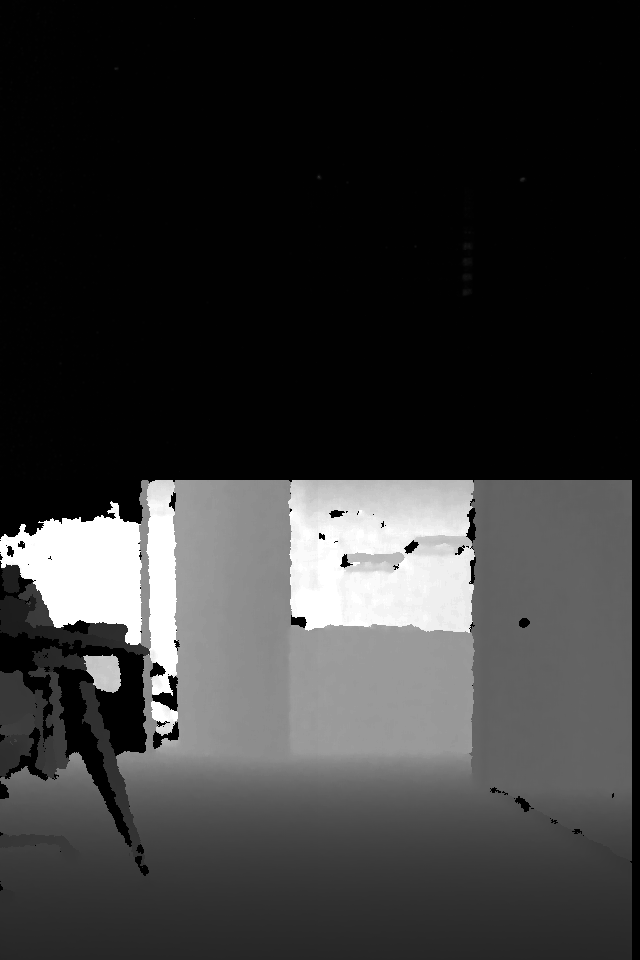
\includegraphics[trim = 0mm 0mm 0mm 0mm, clip, width=\textwidth]{figures/dataset_dark.png}    
        \caption{Dark}
        \label{subfig:dataset_dark}
        \end{subfigure}
        
        \hspace{-3mm}
        \caption{Examplary images belonging to benchmark datasets in different lighting conditions.}
        \label{fig:dataset}
\end{figure}

%----------------------------------------------------------------------------------------------------
% RESULTS
%----------------------------------------------------------------------------------------------------

\section{RESULTS}
\label{sec:results}

\subsection{Detection Performance}

\subsection{Real-Time Performance}

% DISTANCE MATRICES
\begin{figure}[!htb]
        \centering
        
        %%% BRIGHT DISTANCE MATRIX
        \begin{subfigure}[b]{0.27\textwidth}
        \centering
         % trim parameters by order: left, bottom, right, top
        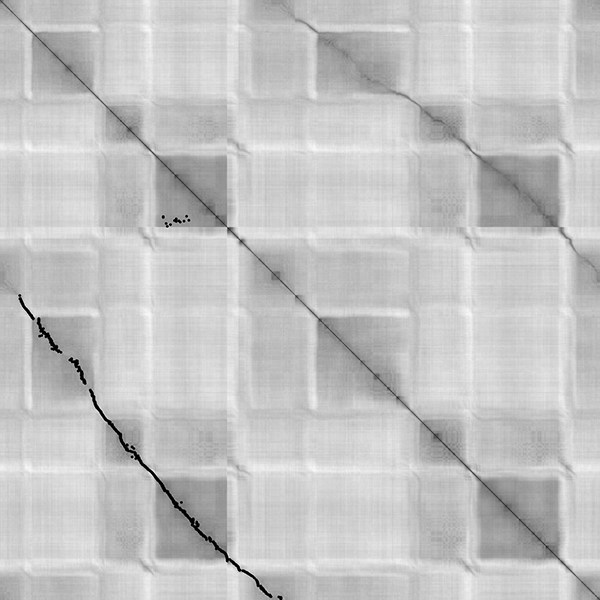
\includegraphics[trim = 0mm 0mm 0mm 0mm, clip, width=\textwidth]{figures/dist_bright.png}    
        \caption{Bright distances}
        \label{subfig:dist_bright}
        \end{subfigure}
        ~ 
        %%% DIM DISTANCE MATRIX
        \begin{subfigure}[b]{0.27\textwidth}
        \centering
         % trim parameters by order: left, bottom, right, top
        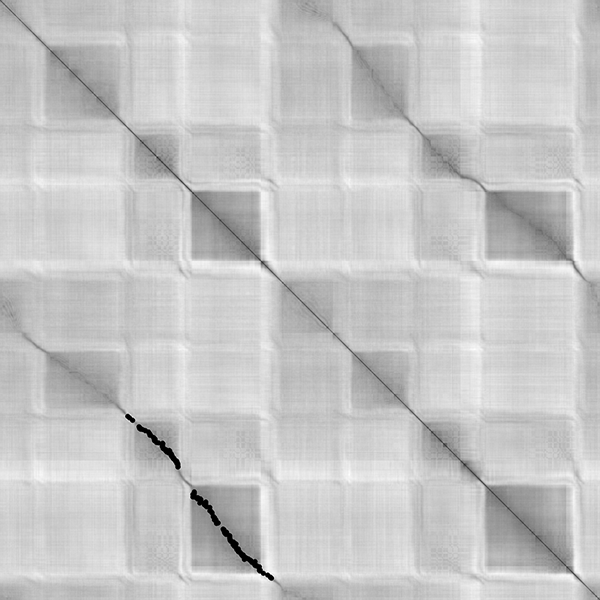
\includegraphics[trim = 0mm 0mm 0mm 0mm, clip, width=\textwidth]{figures/dist_dim.png}    
        \caption{Dim distances}
        \label{subfig:dist_dim}
        \end{subfigure}
         ~ 
        %%% DARK DISTANCE MATRIX
        \begin{subfigure}[b]{0.27\textwidth}
        \centering
         % trim parameters by order: left, bottom, right, top
        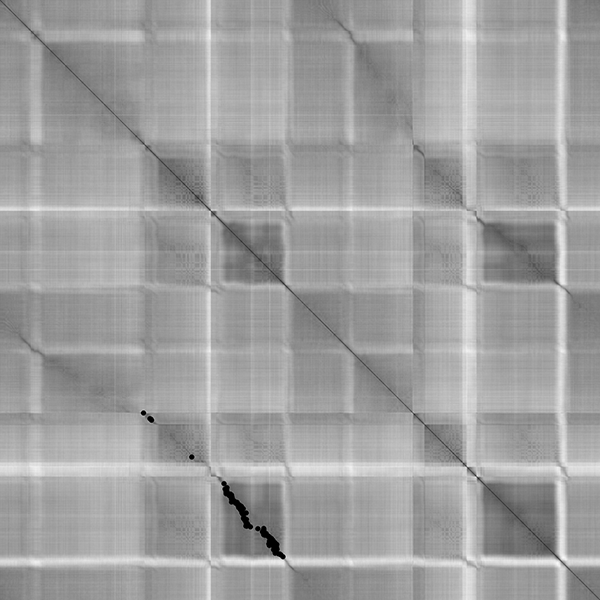
\includegraphics[trim = 0mm 0mm 0mm 0mm, clip, width=\textwidth]{figures/dist_dark.png}    
        \caption{Dark distances}
        \label{subfig:dist_dark}
        \end{subfigure}
        
        \hspace{-3mm}
        \caption{Distance matrixes}
        \label{fig:dist_matrices}
\end{figure}



% RESULTS
\begin{figure}[!htb]
        \centering
        
        %%% BRIGHT PR CURVE
        \begin{subfigure}[b]{0.48\textwidth}
        \centering
         % trim parameters by order: left, bottom, right, top
        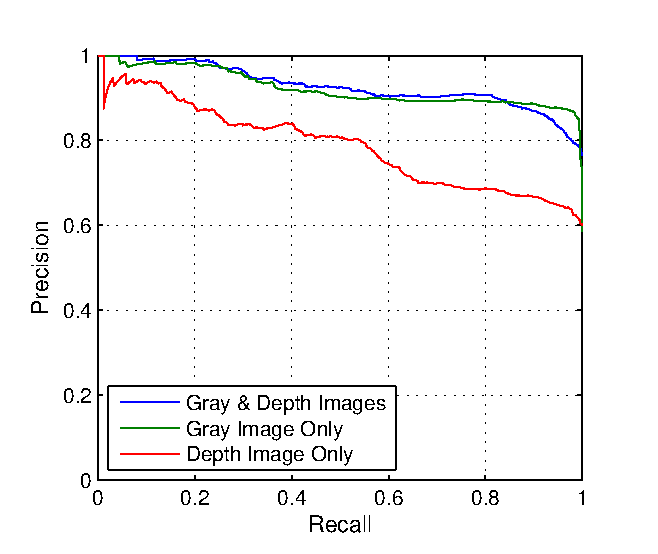
\includegraphics[trim = 0mm 0mm 5mm 0mm, clip, width=\textwidth]{figures/pr_bright.eps}    
        \caption{Bright dataset results.}
        \label{subfig:pr_bright}
        \end{subfigure}
        ~ 
        %%% DIM PR CURVE
        \begin{subfigure}[b]{0.48\textwidth}
        \centering
         % trim parameters by order: left, bottom, right, top
        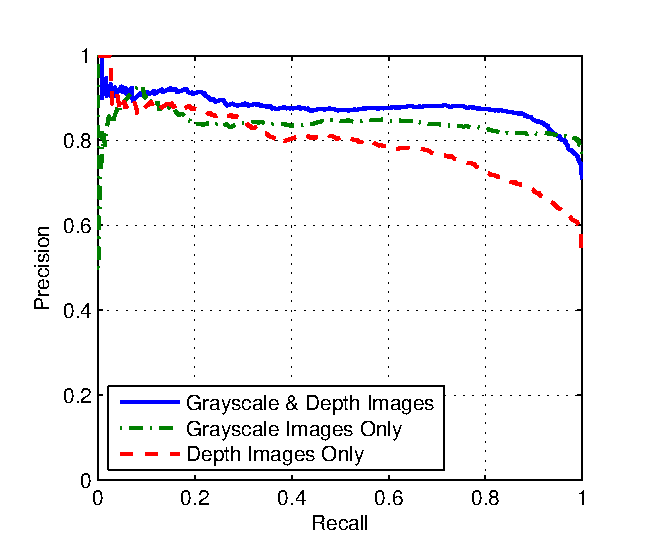
\includegraphics[trim = 0mm 0mm 5mm 0mm, clip, width=\textwidth]{figures/pr_dim.eps}    
        \caption{Dim dataset results.}
        \label{subfig:pr_dim}
        \end{subfigure}
        ~
        %%% DARK PR CURVE
        \begin{subfigure}[b]{0.48\textwidth}
        \centering
         % trim parameters by order: left, bottom, right, top
        \includegraphics[trim = 0mm 0mm 5mm 0mm, clip, width=\textwidth]{figures/pr_dark.eps}    
        \caption{Dark dataset results.}
        \label{subfig:pr_bright}
        \end{subfigure}
        ~ 
        %%% ALL PR CURVE
        \begin{subfigure}[b]{0.48\textwidth}
        \centering
         % trim parameters by order: left, bottom, right, top
        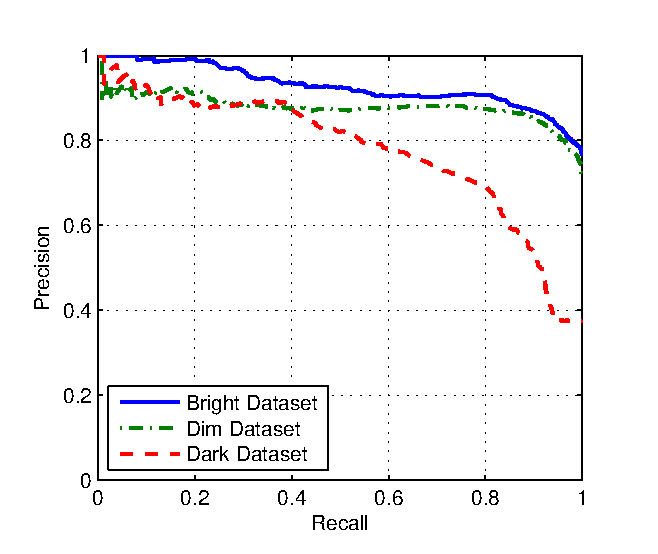
\includegraphics[trim = 0mm 0mm 5mm 0mm, clip, width=\textwidth]{figures/pr_all.eps}    
        \caption{Comparison between datasets.}
        \label{subfig:pr_dim}
        \end{subfigure}

        \hspace{-3mm}
        \caption{PR curves}
        \label{fig:pr_curves}
\end{figure}



%----------------------------------------------------------------------------------------------------
% CONCLUSION AND FUTURE WORK
%----------------------------------------------------------------------------------------------------

\section{CONCLUSION AND FUTURE WORK}

%----------------------------------------------------------------------------------------------------
% ACKNOWLEDGEMENTS
%----------------------------------------------------------------------------------------------------

\acknowledgments         

%----------------------------------------------------------------------------------------------------
% REFERENCES
%----------------------------------------------------------------------------------------------------

\bibliography{report}   % bibliography data in report.bib
\bibliographystyle{spiebib} 

\end{document} 








%----------------------------------------------------------------------------------------------------
% % % % % % % % % % % % % % % % % % % % % % % % COMMENTED 
%----------------------------------------------------------------------------------------------------

\begin{comment}

This document shows the desired format and appearance of a manuscript prepared for the Proceedings of the SPIE.\footnote{The basic format was developed in 1995 by Rick Herman (SPIE) and Ken Hanson (Los Alamos National Lab.).} It is prepared using LaTeX2e\cite{Lamport94} with the class file {\tt spie.cls}.  The LaTeX source file used to create this document is {\tt article.tex}, which contains important formatting information embedded in it.  These files are available on the Internet at {\tt http://home.lanl.gov/kmh/spie/}.  The font used throughout is the LaTeX default font, Computer Modern Roman, which is equivalent to the Times Roman font available on many systems.  If this font is not available, use a similar serif font.  Normal text has a font size of 10 points\footnote{Font sizes are specified in points, abbreviated pt., which is a unit of length.  One inch = 72.27 pt.; one cm = 28.4 pt.} for which the actual height of a capital E is about 2.4 mm (7 pt.) and the line-to-line spacing is about 4.2 mm (12 pt.).  The font attributes for other parts of the manuscript, summarized in Table~\ref{tab:fonts}, are described in the following sections.  Normal text should be justified to both the left and right margins.  Appendix~\ref{sec:latex} has information about PostScript fonts.

To be properly reproduced in the Proceedings, all text and figures must fit inside a rectangle 6.75-in.\ wide by 8.75-in.\ high or 17.15 cm by 22.23 cm.  The text width and height are set in {\tt spie.cls} to match this requirement.
%% This table is carefully placed in the source file to make 
%% it appear at bottom of page, but above the footnotes.  
%% Use of [h] in following command forces table to appear "here".
\begin{table}[h]
\caption{Fonts sizes to be used for various parts of the manuscript.  All fonts are Computer Modern Roman or an equivalent.  Table captions should be centered above the table.  When the caption is too long to fit on one line, it should be justified to the right and left margins of the body of the text.} 
\label{tab:fonts}
\begin{center}       
\begin{tabular}{|l|l|} %% this creates two columns
%% |l|l| to left justify each column entry
%% |c|c| to center each column entry
%% use of \rule[]{}{} below opens up each row
\hline
\rule[-1ex]{0pt}{3.5ex}  Article title & 16 pt., bold, centered  \\
\hline
\rule[-1ex]{0pt}{3.5ex}  Author names and affiliations & 12 pt., normal, centered   \\
\hline
\rule[-1ex]{0pt}{3.5ex}  Section heading & 11 pt., bold, centered (all caps)  \\
\hline
\rule[-1ex]{0pt}{3.5ex}  Subsection heading & 11 pt., bold, left justified  \\
\hline
\rule[-1ex]{0pt}{3.5ex}  Sub-subsection heading & 10 pt., bold, left justified  \\
\hline
\rule[-1ex]{0pt}{3.5ex}  Normal text & 10 pt., normal  \\
\hline
\rule[-1ex]{0pt}{3.5ex}  Figure and table captions & \, 9 pt., normal \\
\hline
\rule[-1ex]{0pt}{3.5ex}  Footnote & \, 9 pt., normal \\
\hline 
\end{tabular}
\end{center}
\end{table} 
The text should begin 1.00 in.\ or 2.54 cm from the top of the page.  The right and left margins should be 0.875~in.\ or 2.22 cm for US letter-size paper (8.5 in.\ by 11 in.) or 1.925 cm for A4 paper (210 mm by 297 mm) to horizontally center the text on the page.  See Appendix~\ref{sec:latex} for guidance regarding paper-size specification. 

Authors are encouraged to follow the principles of sound technical writing, as described in Refs.~\citenum{Alred03} and \citenum{Perelman97}, for example.  Many aspects of technical writing are addressed in the {\em AIP Style Manual}, published by the American Institute of Physics.  It is available on line at {\tt http://www.aip.org/pubservs/style/4thed/toc.html} or {\tt http://public.lanl.gov/kmh/AIP\verb+_+Style\verb+_+4thed.pdf}. A spelling checker is helpful for finding misspelled words. 

An author may use this LaTeX source file as a template by substituting his/her own text in each field.  This document is not meant to be a complete guide on how to use LaTeX.  For that, refer to books on LaTeX usage, such as the definitive work by Lamport\cite{Lamport94} or the very useful compendium by Mittelbach et al.\cite{Mittelbach04}

%%%%%%%%%%%%%%%%%%%%%%%%%%%%%%%%%%%%%%%%%%%%%%%%%%%%%%%%%%%%%
\section{PARTS OF MANUSCRIPT} 

This section describes the normal structure of a manuscript and how each part should be handled.  The appropriate vertical spacing between various parts of this document is achieved in LaTeX through the proper use of defined constructs, such as \verb|\section{}|.  In LaTeX, paragraphs are separated by blank lines in the source file. 

At times it may be desired, for formatting reasons, to break a line without starting a new paragraph.  This situation may occur, for example, when formatting the article title, author information, or section headings.  Line breaks are inserted in LaTeX by entering \verb|\\| or \verb|\linebreak| in the LaTeX source file at the desired location.  

%%%%%%%%%%%%%%%%%%%%%%%%%%%%%%%%%%%%%%%%%%%%%%%%%%%%%%%%%%%%%
\section{SECTION FORMATTING} \label{sec:sections}

Section headings are centered and formatted completely in uppercase 11-point bold font.  Sections should be numbered sequentially, starting with the first section after the Abstract.  The heading starts with the section number, followed by a period.  In LaTeX, a new section is created with the \verb|\section{}| command, which automatically numbers the sections.

Paragraphs that immediately follow a section heading are leading paragraphs and should not be indented, according to standard publishing style\cite{Lamport94}.  The same goes for leading paragraphs of subsections and sub-subsections.  Subsequent paragraphs are standard paragraphs, with 14-pt.\ (5 mm) indentation.  An extra half-line space should be inserted between paragraphs.  In LaTeX, this spacing is specified by the parameter \verb|\parskip|, which is set in {\tt spie.cls}.  Indentation of the first line of a paragraph may be avoided by starting it with \verb|\noindent|.
 
%%-----------------------------------------------------------
\subsection{Subsection Attributes} 

The subsection heading is left justified and set in 11-point, bold font.  Capitalization rules are the same as those for book titles.  The first word of a subsection heading is capitalized.  The remaining words are also capitalized, except for minor words with fewer than four letters, such as articles (a, an, and the), short prepositions (of, at, by, for, in, etc.), and short conjunctions (and, or, as, but, etc.).  Subsection numbers consist of the section number, followed by a period, and the subsection number within that section.  

%%-----------
\subsubsection{Sub-subsection attributes} 
The sub-subsection heading is left justified and its font is 10 point, bold.  Capitalize as for sentences.  The first word of a sub-subsection heading is capitalized.  The rest of the heading is not capitalized, except for acronyms and proper names.  

%%%%%%%%%%%%%%%%%%%%%%%%%%%%%%%%%%%%%%%%%%%%%%%%%%%%%%%%%%%%%
\section{FIGURES AND TABLES} 

Figures are numbered in the order of their first citation.  They should appear in numerical order and on or after the same page as their first reference in the text.  Alternatively, all figures may be placed at the end of the manuscript, that is, after the Reference section.  It is preferable to have figures appear at the top or bottom of the page.  Figures, along with their captions, should be separated from the main text by at least 0.2 in.\ or 5 mm.  

Figure captions are centered below the figure or graph.  Figure captions start with the figure number in 9-point bold font, followed by a period; the text is in 9-point normal font; for example, ``{\footnotesize{Figure 3.}  Original image...}".  See Fig.~\ref{fig:example} for an example of a figure caption.  When the caption is too long to fit on one line, it should be justified to the right and left margins of the body of the text.  

Tables are handled identically to figures, except that their captions appear above the table. 
%%  Use following command to specify that graphics file is in 
%%  a directory other than this LaTeX source file.
%%  Note use of / to separate subdirectories, for UNIX and Windows OS.
%%\graphicspath{{H:/HANSON/SPIESTY/}}
%% tabular environment useful for creating an array of images  
%-------------
   \begin{figure}
   \begin{center}
   \begin{tabular}{c}
   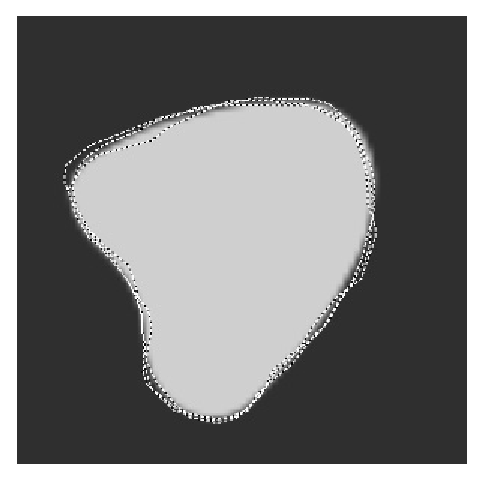
\includegraphics[height=7cm]{figures/mcr3b.eps}
   \end{tabular}
   \end{center}
   \caption[example] 
%>>>> use \label inside caption to get Fig. number with \ref{}
   { \label{fig:example} 
Figure captions are used to describe the figure and help the reader understand it's significance.  The caption should be centered underneath the figure and set in 9-point font.  It is preferable for figures and tables to be placed at the top or bottom of the page. LaTeX tends to adhere to this standard.}
   \end{figure} 
%-------------

For further details concerning the inclusion of grayscale and color images, consult SPIE's {\it Author Guide for Publication and Presentation}.
 
%%%%%%%%%%%%%%%%%%%%%%%%%%%%%%%%%%%%%%%%%%%%%%%%%%%%
\appendix    %>>>> this command starts appendixes
%%%%%%%%%%%%%%%%%%%%%%%%%%%%%%%%%%%%%%%%%%%%%%%%%%%%
\section{MISCELLANEOUS FORMATTING DETAILS} \label{sec:misc}

It is often useful to refer back (or forward) to other sections in the article.  Such references are made by section number.  When a section reference starts a sentence, Section is spelled out; otherwise use its abbreviation, for example, ``In Sec.~2 we showed..." or ``Section~2.1 contained a description...".  References to figures, tables, and theorems are handled the same way.

At the first occurrence of an acronym, spell it out, followed by the acronym in parentheses, e.g., noise power spectrum (NPS).  
 
%%-----------------------------------------------
\subsection{Formatting Equations} 
Equations may appear in line with the text, if they are simple, short, and not of major importance; e.g., $\beta = b/r$.  Important equations appear on their own line.  Such equations are centered.  For example, ``The expression for the minus-log-posterior is
	\begin{equation}
	\label{eq:alpha}
\phi = |{\rm\bf y} - {\rm\bf A}{\rm\bf x}|^2 + \alpha \log p({\rm\bf x}) \, ,
	\end{equation}
where $\alpha$ determines the strength of ..."  Principal equations are numbered, with the equation number placed within parentheses and right justified.  

Equations are considered to be part of a sentence and should be punctuated accordingly. In the above example, a comma follows the equation because the next line is a subordinate clause.  If the equation ends the sentence, a period should follow the equation.  The line following an equation should not be indented unless it is meant to start a new paragraph.  Indentation after an equation is avoided in LaTeX by not leaving a blank line between the equation and the subsequent text.

References to equations include the equation number in parentheses, for example, ``Equation~(\ref{eq:alpha}) shows ..." or ``Combining Eqs.~(2) and (3), we obtain..."  Using a tilde in the LaTeX source file between two characters avoids unwanted line breaks.

%%-----------------------------------------------------------
\subsection{Formatting Theorems} 

To include theorems in a formal way, the theorem identification should appear in a 10-point, bold font, left justified and followed by a period.  The text of the theorem continues on the same line in normal, 10-point font.  For example, 

\noindent{\bf Theorem 1.} For any unbiased estimator...

Formal statements of lemmas and algorithms receive a similar treatment.

%%%%%%%%%%%%%%%%%%%%%%%%%%%%%%%%%%%%%%%%%%%%%%%%%%%%
\section{SOME LATEX GUIDANCE} \label{sec:latex}

%%-----------------------------------------------------------
\subsection{Margins and PostScript Fonts}
 
Manuscripts submitted electronically to as PostScript (PS) files must have the correct margins. LaTeX margins are related to the document's paper size. The paper size is set at two separate places in the process of creating a PS file. The first place is in {\tt latex}. The default in {\tt article.tex}, on which {\tt spie.cls} is based, is USA letter paper. To format a document for A4 paper, the first line of the LaTeX source file should be \verb|\documentclass[a4paper]{spie}|.   

The output of the LaTeX utility is a file with the extension DVI (for Device Independent), which encodes the formatted document.  The application DVIPS is typically used to convert the DVI file to a PS file.  DVIPS has its own default paper size, which can be overridden with the option ``{\tt -t letter}" or ``{\tt -t a4}".  
If the foregoing steps do not produce the correct top margin, you can move the text lower on the page (by 9 mm) with the command \verb|\addtolength{\voffset}{9mm}|, placed right after the \verb|\documentclass| command, for example.

Another DVIPS option specifies the incorporation of (scalable) PostScript Type 1 fonts in its output PS file. This feature is important for obtaining a subsequent PDF file that will be clearly displayed on a computer monitor by Adobe Acrobat Reader.  The option ``{\tt -P pdf}" makes DVIPS include these fonts in its output PS file.

%%-----------------------------------------------------------
\subsection{Bold Math Symbols} 

The math package from the American Mathematical Society allows one to easily produce bold math symbols, well beyond what is available in LaTeX. It also provides many useful capabilities for creating elaborate mathematical expressions. You need to load the AMS math package near the top of the LaTeX source file, right after the \verb+\documentclass+ command:\\[1ex]
\verb+\usepackage[]{amsmath}+ \\[1ex]
Then for bold math symbols use \verb+\boldsymbol+ in equations, e.g., 
\verb+$\boldsymbol{\pi}$+ 
yields a bold pi.  You can make it easier to use by defining a command:\\[1ex]
\verb+\newcommand{\bm}[1]{\boldsymbol{#1}}+ \\[1ex]
and then using it like so \verb+$\bm{\pi}$+.

Not all math symbols are available in bold.  In a pinch, you can use \verb+\pmb+ ("poor man's bold"), which is defined in \verb+amsmath+. This command approximates a bold character with a superposition of several, slightly displaced unbold characters.

If you want a Greek symbol in the article title, it should be both larger and bold. The easiest thing is to load the AMS math package as described above. 
Then, in the title, use something like:\\[1ex]
\verb+\title{Estimation of {\LARGE$\boldsymbol\alpha$} by a Monte Carlo technique}+ \\[1ex]
Note that the command to create the alpha character is enclosed within braces to form a self-contained environment. The use of \verb+\LARGE+ in this example may not be needed when using nondefault font packages, such as the {\tt times} package, because of how the article title is handled in {\tt spie.cls}.

%%-----------------------------------------------------------
\subsection{Uppercase letters and special symbols in BibTex} 

BibTeX tries to enforce standard publishing rules regarding article titles and authors' names; it sometimes changes uppercase letters to lower case. BibTeX also has trouble with umlauts, generally created in LaTeX with \verb+\"{o}+, because it is looking for the \verb+"+ to end the input line. 

The general rule for overriding LaTeX's and BibTex's reinterpretation of your input text is to put the items you wish to be unchanged in braces. Thus, to obtain an umlaut in an author's name or in an article title, or to force an uppercase letter, do something like the following: \\[1ex]
\verb+ @article{Kaczmarz37,+ \\ 
\verb+ author = "S. Kaczmarz",+ \\ 
\verb+ title  = "Angen{\"{a}}hrte {A}ufl{\"{o}}sung von {S}ystemen linearer {G}leichungen",+ \\ 
\verb+ journal= "Bull. Acad. Polon. Sci. Lett.",+ \\ 
\verb+ volume = "A35",+ \\ 
\verb+ pages  = "355-357",+ \\	
\verb+ year   = "1937"	} + \\[1ex]
This example shows the use of both umlauts and uppercase letters.

\end{comment}
